 %!TEX root = main.tex
\chapter{Random walks and diffusion}

In absence of active transport, microscopic objects move due to ubiquitous thermal motion:
Every molecule jitters around in random ways and the sum of the many kicks and pushes causes an erratic movement known as \href{https://en.wikipedia.org/wiki/Brownian_motion}{Brownian motion}.
It is named after Robert Brown who noticed that pollen grains jitter when observing them in a microscope.
Such Brownian motion or diffusion is the primary mode at which nutrients, signaling molecules, and proteins move around in bacterial cells.
In this chapter, we will explore the basic properties of diffusion and how it depends on the size of the particles, the viscosity of the medium, and temperature.

Getting a sense of the time scales over which molecules diffuse certain distances is crucial for a quantitative understanding of many biological process.
The process of diffusion of molecules in the cytosol can be studied and quantified using the technique \href{https://en.wikipedia.org/wiki/Fluorescence_recovery_after_photobleaching}{``Fluorescence Recovery After Photobleaching''} (FRAP), see Fig.~\ref{fig:FRAP}
Say you labeled your molecule of interest with a fluorescent protein (GFP) that bleaches due to photo damage in strong illumination.
If you now bleach the dye in some fraction of your field of view, you have set up a sharp gradient between fluorescent and non-fluorescent versions of your molecule.
The recovery of the fluorescence signal is due to diffusion of intact GFP molecules into the space that was bleached.
This fluorescent recovery is very smooth and deterministic, despite the fact that the motion of the individual particles is completely erratic and random.
This is just one example how the net effect of many random events gives rise to behavior that is simple and smooth.
We will explore how this comes about in the next section.

\begin{figure}[tb]
	\centering
	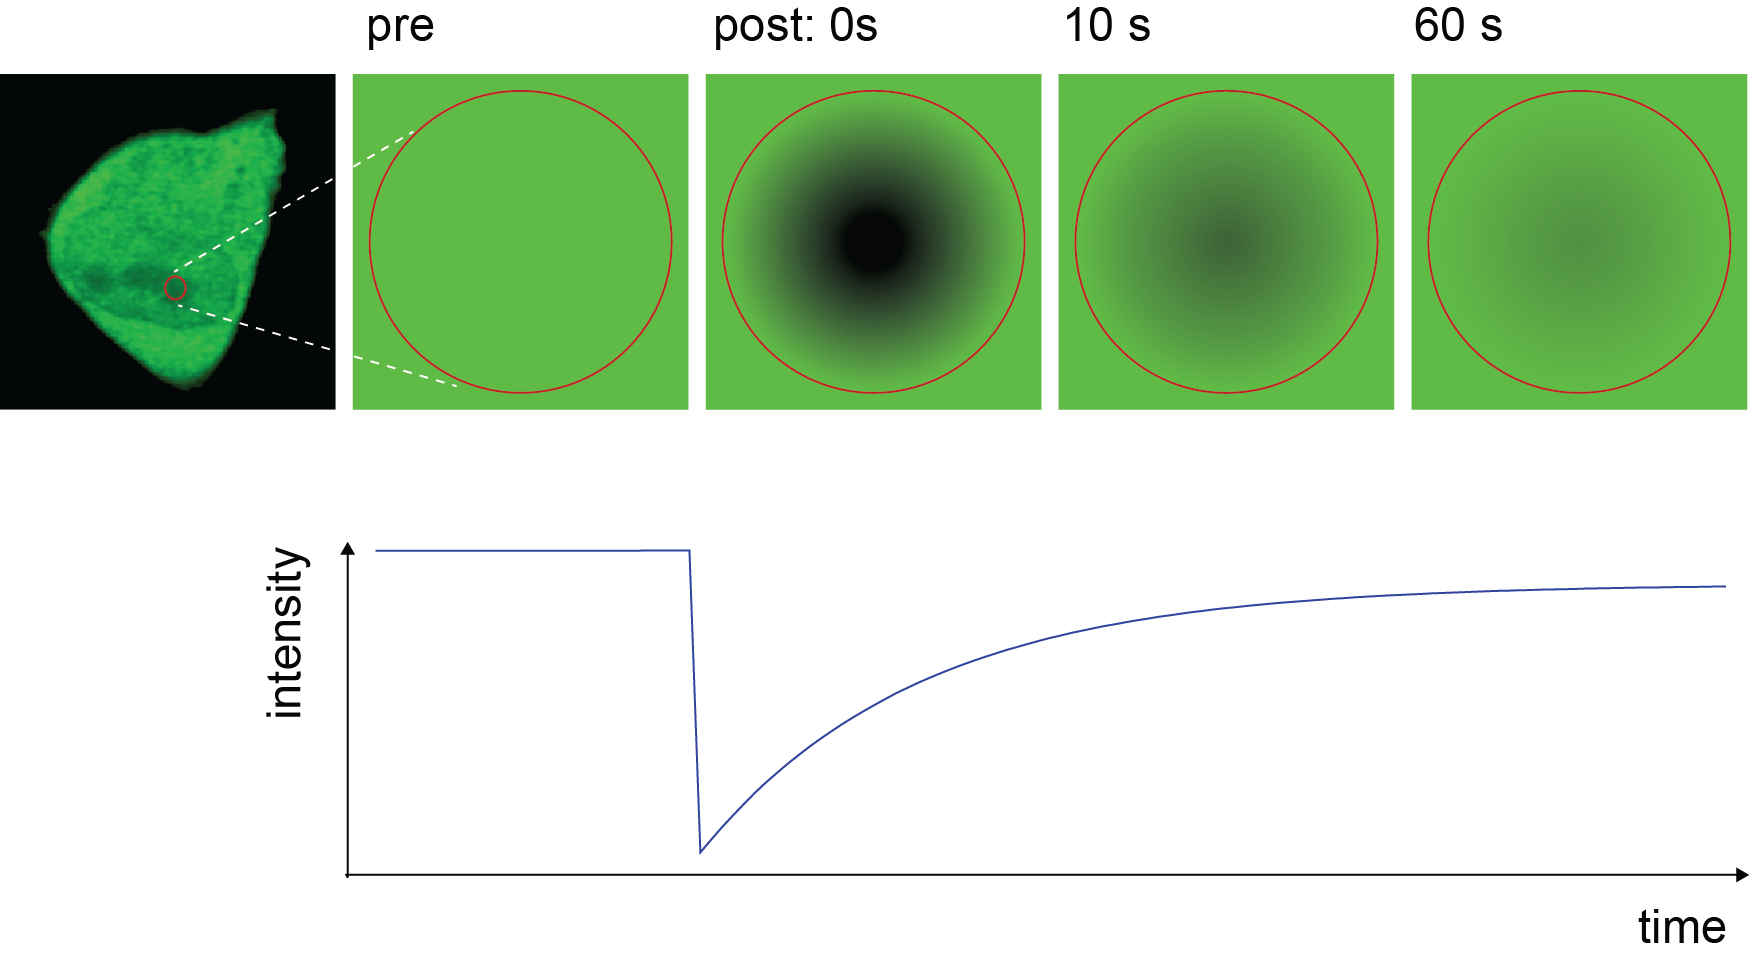
\includegraphics[width=\textwidth]{FRAP.png}
	\caption{The top left image shows a cell with GFP at homogeneous concentration in the cytosol. After bleaching (destroying) the fluorescent proteins in small volume with a high intensity laser, fluorescence recovers overtime through diffusion of intact GFP into the bleached volume.  Image source: bioquant Heidelberg}
	\label{fig:FRAP}
\end{figure}

\section{Random walks in one dimension}
Consider an object on a track that moves by a fixed distance every second.
With probability $p$ is moves to the right and with probability $q=1-p$ it moves to the left.
How far do expect this object to be after $n=1,10,100,\dots$ steps?
This simple example has a closed solution, but we will explore this with a little simulation before going into the math.
Take a look at the little code snippet \ref{lst:random_walk}.
This code generates a couple of random walks and graphs them.
A typical output is shown in Fig.~\ref{fig:RW}.

\begin{listing}[h]
\inputminted{python}{scripts/random_walk.py}
\caption{Script that generates and plots random walks.}
\label{lst:random_walk}
\end{listing}

\begin{figure}[tb]
	\centering
	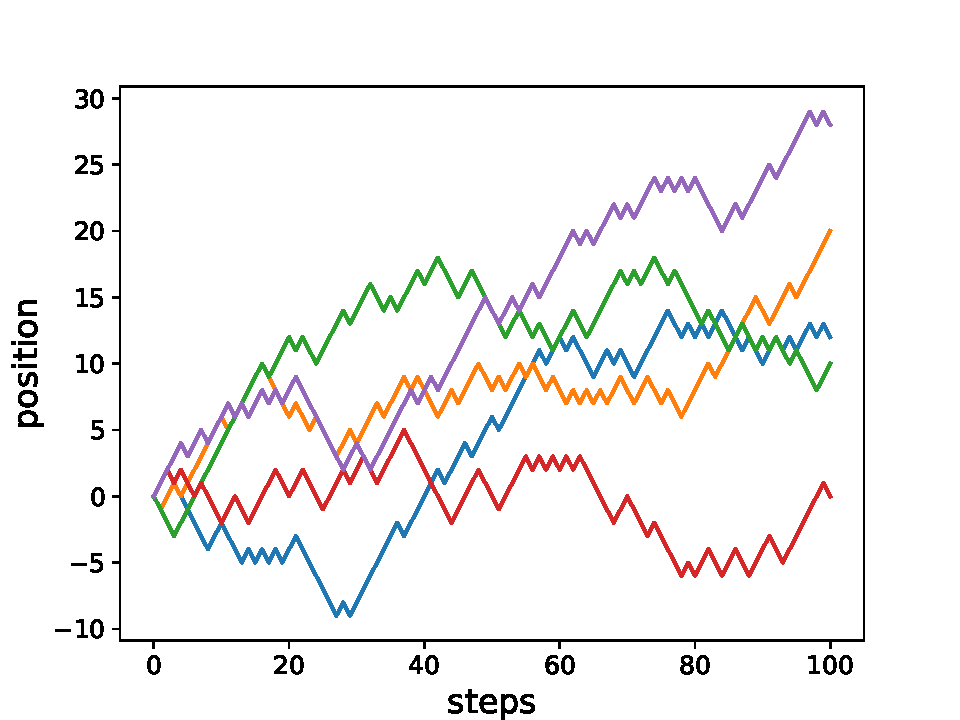
\includegraphics[width=0.48\textwidth]{figures/random_walk.pdf}
	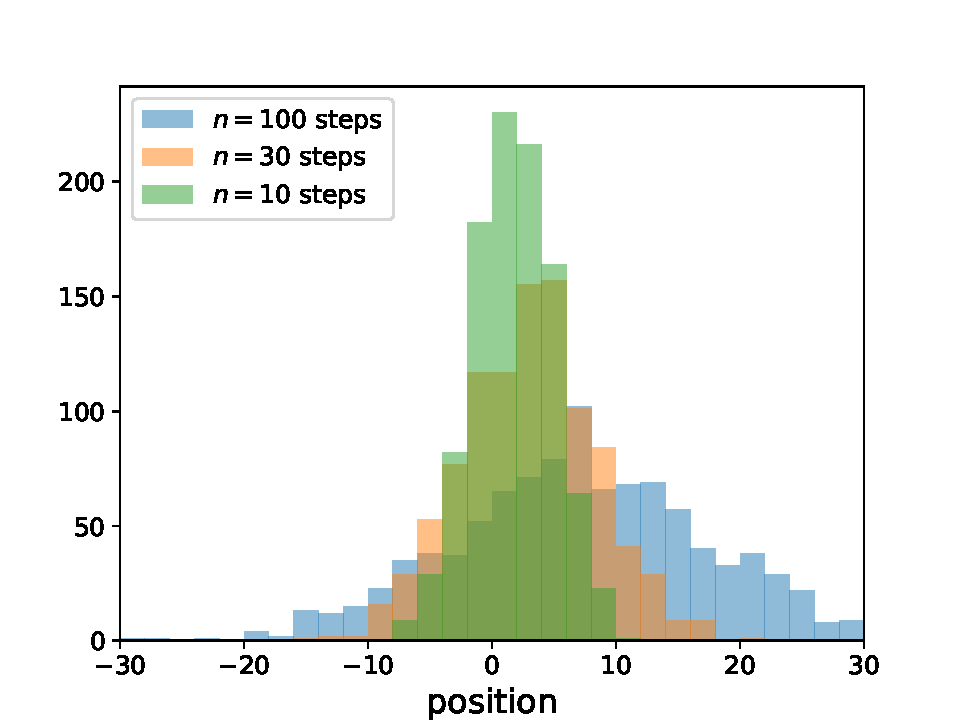
\includegraphics[width=0.48\textwidth]{figures/random_walk_histogram.pdf}
	\caption{Left: 5 realizations of a random walk with $p=0.53$. Right: Histograms of the position of random walks after $n=10, 30, 100$ steps. The histograms are getting wider and slowly move to the right. }
	\label{fig:RW}
\end{figure}

After having explored such random walks in simulations, let's look at them more systematically.
The probability of a particular sequence of left/right steps is $p^k q^{n-k}$, where $k$ is the number of steps to the right and $n-k$ is the number of steps to the left.
Now there is exactly one way of taking $n$ out of $n$ steps to the right or left, but there are many ways of doing some mix of right/left steps.
In fact, the number of ways to walk $k$ steps to the right and $n-k$ steps to the left is given by
\begin{equation}
	C_n^k = \frac{n!}{k!(n-k)!} = { n\choose k}
\end{equation}
This is known as the binomial coefficient and should be familiar from high-school.
The factorial $n! = n(n-1)(n-2)\cdots 2\cdot1$
The probability of observing the random walk at position $k$ is therefore given by
\begin{equation}
	P_n^k = p^kq^{n-k}\frac{n!}{k!(n-k)!}
\end{equation}
which is known as the Binomial Distribution.

\subsection{Mean and variance of a random walk}
On average, the random walker will move to the right if $p>q$, to the left if $p<q$, and no net movement is expected if $p=q=0.5$.
This intuition is confirmed by a short calculation.
The number of steps to the right is given by
\begin{equation}
\begin{split}
	\langle k \rangle & = \sum_{k=0}^n k P_n^k = \sum_{k=1}^n \frac{n!}{(k-1)! (n-k)!} p^k q^{n-k} \\
	&= np \sum_{k=1}^n \frac{(n-1)!}{(k-1)! (n-k)!} p^{k-1} q^{n-k} = np
\end{split}
\end{equation}
where the last equality used the fact that summand is again a binomial distribution $P(k-1, n-1)$ and hence the sum evaluates to one.
After $n$ steps, the walker has therefore taken on average $np$ steps to the right and $nq$ steps to the left and the average position is therefore $n(p-q)$.

This calculation established that the mean position of the random walker is $\langle x\rangle = n(p-q)$, but random walkers are not moving deterministically along the mean.
Instead, some will be on the left, some of the right of $\langle x\rangle$.
To quantify the spread of a random walk, we calculate its variance.
The variance is defined as the mean squared distance from the mean and we will first calculate the variance in the number of steps to the right.
The details of this calculation are a little tedious, but straightforward, and I provide them at the end of this chapter:
\begin{equation}
	\langle (k - np)^2 \rangle = \sum_{k=0}^n k^2 P_n^k - n^2p^2 = npq
\end{equation}
Since the $x=2k-n$ we immediately find $var(x) = 4npq$.
Note that this is the average squared deviation from the mean.
The typical distance from the mean is therefore the square root $\delta x \sim 2\sqrt{npq}$.
The fact that the typically spread of the random walker increases with the square root of the number of steps has far reaching implications.
In particular, the random component of the motion dominates initially
\begin{equation}
	2\sqrt{npq} > n(p-q) \quad \Rightarrow \quad n < \frac{4pq}{(p-q)^2}
\end{equation}
The smaller the difference between $p$ and $q$, the longer the random part dominates.
If $p$ is very close to $q$, the random part dominates for a very long time!
The fact that random components depend on the square root of the number events/steps/experiments while the deterministic part is linear in this number is the basis of almost all statistical tests and you will encounter this relationship over and over again.

It is important to realize that in most situations, the probability to move to the right or the left are exactly the same: When there is no force pulling the molecule in a particular direction, thermal noise will move it in every direction with equal rate.
In this case, $\langle x \rangle = 0$ no matter how long you wait and the only contribution to a molecules motion is the random component $2\sqrt{npq}$.

\subsection{From random walks to diffusion}
So far, we discussed the properties of random walks on a discrete one dimensional grid.
The equation describing the distribution of this random walk can be rewritten as
\begin{equation}
	P(x,n) = p P(x-1,n-1) + q P(x+1,n-1)
\end{equation}
This equation describes how the probability of finding the walker at position $x$ changes with every step: the first term involves a step to the right which happens with probability $p$, the second term corresponds to a step to the left.

\begin{figure}[tb]
	\centering
	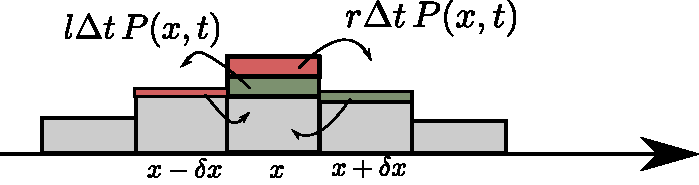
\includegraphics[width=0.6\columnwidth]{figures/RW_masterEq}
	\caption{Schematic of the dynamics of the distribution $P(x,t)$ of the
	position of a diffusing substance. The center bin at $x$ looses mass to the left (red) and right (green) but gains from the bins at $x\pm \delta x$. The neighboring bins, however, are smaller and $P(x,t)$ will therefore decrease. The diffusion equation is obtained by reducing $\delta x$ and $\Delta t$ gradually to 0.}
	\label{fig:masterEQ}
\end{figure}

In a biological system, there are no discrete time points and a molecule will move due to thermal motion by a random distance.
But we can approximate this situation by making the time and spatial steps smaller and smaller.
We will from now on replace $n$ by time $t$ and treat the position $x$ as a continuous variable.
In a time interval $\Delta t$, the molecule receives kicks that push it to the right of left by a distance $\delta x$ with probability $r\Delta t$ and $l\Delta t$.
\begin{equation}
	P(x,t+\Delta t) = (1-(r+l)\Delta t) P(x,t) + r\Delta t P(x-\delta x, t) + l\Delta t P(x+\delta x,t)
\end{equation}
The first term on the right hand side corresponds to cases where the molecular stays where it is.
The second and third term correspond to jitter to the right and left, respectively (see Figure \ref{fig:masterEQ}).
This equation can be rearranged slightly
\begin{equation}
	\frac{P(x,t+\Delta t) - P(x,t)}{\Delta t} = -(r+l) P(x,t) + r P(x-\delta x, t) + l P(x+\delta x,t)
\end{equation}
which should remind you of a differential equation.
Rearranging this a little more, we find
\begin{equation}
\begin{split}
	\label{eq:discrete_update}
	\frac{P(x,t+\Delta t) - P(x,t)}{\Delta t} = &\frac{\delta x^2(r+l)}{2} \frac{P(x+\delta x,t) - 2 P(x,t) +P(x-\delta x, t)}{\delta x^2}\\&
	 - \delta x (r-l) \frac{P(x+\delta x, t) - P(x-\delta x,t)}{2\delta x}
\end{split}
\end{equation}
The terms on the right hand site are discrete second and frist derivatives (see \href{https://en.wikipedia.org/wiki/Finite_difference}{Finite differences} on wikipedia).
Defining the diffusion coefficient $D=\frac{\delta x^2 (r+l)}{2}$, the drift velocity $v=\delta x (r-l)$, and taking the limit of small space and time steps, we arrive at
\begin{equation}
\label{eq:diffusion}
	\frac{\partial P(x,t)}{\partial t} = D\frac{\partial^2 P(x,t)}{\partial x^2} - v \frac{\partial P(x,t)}{\partial x}
\end{equation}
This equation is called diffusion equation and describes transport in many biological systems -- it is also known as the heat equation as it describes the flow of heat in a solid.
This type of equation is called a partial differential equation -- something you might not have come across in previous courses.
The concept is not very difficult, but the different notations that are used for such equations can be confusing (see \href{https://en.wikipedia.org/wiki/Partial_derivative}{wikipedia on partial derivatives}).

The object $P(x,t)$ can be interpreted as the density of molecules at position $x$ and time $t$.
This density changes due to diffusion of the molecules according to Eq.~\ref{eq:diffusion}.
For the following discussion, we will assume that $v=0$, that is there is no directed motion.
In this case, density increase were curvatures is positive and decreases where it is negative.
In other words, ``hills'' decrease and ``valleys'' are filled.

The diffusion constant $D$ has units of length${}^2$/time, e.g.~m$^2$/s.
Even though the diffusion constant determines how rapidly molecules spread, it is not a velocity which would have units m/s.
The crucial difference is that diffusion describes \emph{undirected} motion, while velocities describe directed motion.
Undirected motion has to be characterized in terms of the squared displacement since the net displacement vanishes.


\subsubsection{Solutions to the diffusion equation}
In our discussion of discrete random walks, we showed that the binomial distribution describes the position of the walker after $n$ steps.
You might know that the continuous analog of the binomial distribution is the {\it Gaussian} or {\it Normal} distribution.
A normal distribution (centered around $x=0$) with variance $\sigma^2$ is given by
\begin{equation}
	N(x | \sigma) = \frac{1}{\sqrt{2\pi \sigma^2}} e^{\frac{x^2}{2\sigma^2}}
\end{equation}
The normal distribution is a solution to the diffusion equation with
\begin{equation}
	\sigma^2 = 2Dt
\end{equation}
This can be readily verified by direct computation and is done explicitly at the end of this chapter.

\subsubsection{Numerical solution of the diffusion equation}
In many cases, analytical solution of the diffusion equation is not possible and one instead resorts to numerical methods.
Numerical solutions essentially work with the discrete approximation Eq.~\ref{eq:discrete_update}.
The hopping rates $r$ and $l$ depend on $D$ and $v$ (independent of the discretization) and the spatial discretization:
\begin{equation}
	D = \frac{r+l}{2}\delta x^2 \quad \mathrm{and} \quad v =(r-l)\delta x
\end{equation}
is readily solved for $r$ and $l$
\begin{equation}
	l = \frac{D}{\delta x^2}- \frac{v}{2\delta x}\quad \mathrm{and} \quad
	r = \frac{D}{\delta x^2} + \frac{v}{2\delta x}
\end{equation}

\subsection{Typical diffusion coefficients in cells}

\begin{itemize}
  \item GFP in eukaryotic cells: $\sim 25 \mu m^2/s$
  \item GFP in prokaryotic cells: $\sim 10 \mu m^2/s$
  \item mRNA (actin in mouse): $\sim 0.2 \mu m^2/s$
  \item $\mathrm{H_2O}$ molecule in $\mathrm{H_2O}$: $\sim 2000 \mu m^2/s$
  \item $\mathrm{H^+}$ molecule in $\mathrm{H_2O}$: $\sim 7000 \mu m^2/s$
\end{itemize}


\subsubsection{How long does it take for a protein to diffuse a distance $x$?}
The typical distance scale after a time $t$ is
\begin{equation}
	\Delta x = \sqrt{2Dt} \quad \Rightarrow \quad t = \frac{\Delta x^2}{2D}
\end{equation}

\begin{itemize}
  \item $\Delta x = 1\mu m$: $t = 0.05s$ [across a bacterium]
  \item $\Delta x = 10\mu m$: $t = 5s$   [across a eukaryotic cell]
  \item $\Delta x = 1000\mu m$: $t = 5000s=83m$
  \item $\Delta x = 1m$: $t = 5\times 10^9s=160y$   [along a peripheral axon]
\end{itemize}
Hence diffusion is fast on short distances, but completely inadequate on long distances.


\section{Fluxes}
Much transport in biology is diffusive: Many enzymatic rates are diffusion limited and processes like nuclear import involves diffusion through the nuclear pore (facilitated by suitable transport proteins).
We will now explore different ways in which diffusion is mediating and limited such rates.

Consider the set-up illustrated in Fig.~\ref{fig:diffusive_transport} of a long narrow channel with a high concentration on the left and a low concentration on the right.
If the channel is narrow and the reservoirs on the left and right large, we expect an approximately homogeneous concentration in both reservoirs and a steady concentration gradient across the channel.
The diffusion of molecules in our system is governed by the diffusion equation and we there expect that the should be a solution to the diffusion equation that (i) does not depend on time ($P(x,t)=P(x)$), and (ii) that is high on the left, low on the right, and has a gradient in the middle.
The only spatial direction that is relevant in Fig.~\ref{fig:diffusive_transport} is the $x$ axis and we will ignore slight variation long the $y$ and $z$ axes.
A time invariant solution implies
\begin{equation}
	\frac{\partial P(x,t)}{\partial t} = 0 = D\frac{\partial^2 P(x,t)}{\partial x^2} = 0
\end{equation}
This equation tells us two things: (i) the solution has to be independent of $t$, and (ii) is has zero curvature in $x$.
Zero curvature implies that the solutions are linear.
Inside the channel, we therefore have
\begin{equation}
 	P(x) = P^l + \frac{(P^r-P^l)x}{L} \ ,
\end{equation}
where $P^l$ and $P^{r}$ are the concentrations on the left and right while $L$ is the length of the channel and $x$ is the coordinate along the channel $x\in [0,L]$.
Our intuition already tells us that in a set-up like Fig.~\ref{fig:diffusive_transport} material will flow from left to right, that is the concentration on left will decrease slowly while that on the right will increase (in analogy to temperature equilibration).
To calculate this flux, it is useful to rewrite the diffusion equation
\begin{equation}
	\frac{\partial P(x,t)}{\partial t} = -\frac{\partial }{\partial x}\left[-D\frac{\partial P(x,t)}{\partial x} \right] = - \frac{\partial }{\partial x} j(x,t)
\end{equation}
The object in brackets is known as the flux $j(x,t)$.
Once broken down like this, the diffusion equation is rather intuitive: the concentration changes in time if the flux changes in space.

In our case, the material transported across the channel is
\begin{equation}
	J = D\frac{P^l - P^r}{L}\times A
\end{equation}
where $A$ is the cross-sectional area of the channel.
Let's do a quick consistency check: $D$ has units $m^2/s$, concentrations have units $\mathrm{stuff}/m^3$, $L$ has units $m$ and $A$ has units $m^2$. Hence $J$ has units $\mathrm{stuff}/s$ which is exactly what we expect for a flux.

\begin{figure}[tb]
	\centering
	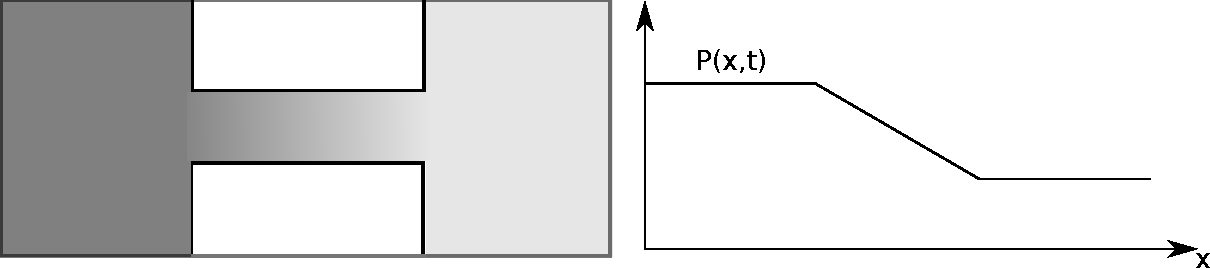
\includegraphics[width=\textwidth]{figures/diffusive_gradient.pdf}
	\caption{Diffusion through a narrow channel between two reservoirs results in a linear concentration profile along the channel.}
	\label{fig:diffusive_transport}
\end{figure}

\subsubsection*{Transport through the nuclear pore}
With these results, we can now estimate the number of molecules that transverse the nuclear pore per second given a concentration gradient.
The center of the nuclear pore has a diameter of about 30nm and a height of about 30nm.
A typical protein has a diffusion coefficient of about $10\mu m^2/s$.
Our expectation for the number of particle translocations is therefore
\begin{equation}
	J \approx \Delta C \times 0.025\mu m^3/s \approx 2.5\times 10^{-16}l/s \Delta C
\end{equation}
At a $\mu M$ concentration difference, this corresponds to a few hundred molecules per second.
There are extremely rough estimates and the medium inside the pore will have significant effects on this number, but we get a first idea.
For more detail on this problem, see this paper by \citet{ribbeck_kinetic_2001}.

\subsubsection*{Diffusion limited rates}
Many biochemical reactions are limited by the time it takes for the reactants to find each other.
Since the reactants move around by diffusion, such rates are called \emph{diffusion limited}.
In this case the activity of an enzyme, for example, cannot be increased by modifying the enzyme since the fundamental speed-limit is the arrival of the substrate.
The rate of reaction, however, will increase with the substrate concentration.
The full solution of this problem involves solving the diffusion equation in three dimensions.
While possible, we don't want to go into these technicalities here and simply state and motivate the result.
The diffusion limited rate between substance $a$ and substance $b$ is given by
\begin{equation}
	\label{eq:diffusion_limit}
	\kappa = 4\pi (D_a+D_b)(r_a+r_b) \ ,
\end{equation}
where $D_a$ and $D_b$ are the diffusion coefficients and $r_a$ and $r_b$ are the radii of the two reactants.
The sum of the two diffusion coefficients happens to be the diffusion of the relative distance between two molecules, and the sum of the radii is the minimal distance the two reactants have to attain to react.
The quantity $\kappa$ as units $m^3/s$, which becomes `particles per second' when multiplied by a concentration.

The situation above is quite idealized and additional factors, for example relative orientation, affect the actual rate.


\section{Diffusion coefficients and Stokes-Einstein relation}
There is simple law that relates the diffusion constant to other properties of the medium and the diffusion particles: this law is called the Stokes-Einstein relation.
Before we derive it, lets take a moment to think about which quantities might matter:
\begin{itemize}
  \item big things diffuse more slowly, hence the radius $r$ with units $length$ is important
  \item diffusion is thermal motion, hence $kT$ with units $energy$ should be relevant
  \item diffusion is slower at high viscosity, hence $\eta$ with units $Force\cdot time/area$ will matter.
  	(viscosity is the factor relating the force per unity area to the velocity gradient in fluid flow.)
\end{itemize}

How can we combine these quantities to give us a diffusion constant with units $length^2/time$?
Clearly, $\eta$ has to be in the denominator and $kT$ in the numerator. Their ratio has the following units:
\begin{equation}
\frac{kT}{\eta}\quad \mathrm{has\ units}\quad \frac{Force\cdot length\cdot area}{Force \cdot time} = \frac{length^3}{time}
\end{equation}
Hence $kT/\eta r$ has the right units and we expect the diffusion coefficient to scale as
\begin{equation}
D \sim \frac{kT}{\eta r}
\end{equation}
Let's see how this holds up when analyzing the problem more carefully.
Einstein considered diffusion in a general potential. We will assume here we have a harmonic potential $U(x) = \alpha x^2/2$, i.e., a force $F = \alpha x$ is pulling the particle back to $x=0$.
The motion of the particle is governed by the diffusion equation
\begin{equation}
\frac{\partial P(x,t)}{\partial t} = D \frac{\partial^2 P(x,t)}{\partial x^2} + \alpha \mu \frac{\partial P(x,t)}{\partial x}
\end{equation}
where $\mu$ is the mobility of the particle, i.e., the relationship between velocity and pulling force in viscous media. Mobility is the inverse of friction.
At steady state, the distribution of the particle is
\begin{equation}
P(x) = \frac{1}{\sqrt{2\pi D/\alpha}}e^{ - \frac{\alpha x^2}{2D}}
\end{equation}
However, the Maxwell-Boltzmann distribution requires that the equilibrium distribution is also proportional to $e^{-\alpha x^2/2kT}$. Hence we find
\begin{equation}
D = \mu kT
\end{equation}
This is one example of a fluctuation-dissipation relation that connects macroscopic quantities such as mobility with the microscopic quantities such as the diffusion coefficients.

Next, we need to consider how the mobility is related to the geometry of the particle and the solution.
This is given by Stokes' law (see Section \ref{sec:stokeslaw}) that relates the friction force to the size of the sphere and the viscosity:
\begin{equation}
\mu = \frac{1}{6\pi \eta r}
\end{equation}
Deriving this is a standard exercise in fluid dynamics, but nothing that we will go into here. Have a look at \href{https://en.wikipedia.org/wiki/Stokes%27_law}{the wikipedia page for Stokes' law} if you are curious.

Putting the Einstein relation and Stokes' law together, we obtain the Stokes-Einstein relation
\begin{equation}
D = \frac{kT}{6\pi \eta r}
\end{equation}
The remarkable fact about this equation is that $\eta$ can be measured at macroscopic scales and the microscopic structure does not feature explicitly. Nevertheless, together with the molecular radius and the energy scale $kT$, it determines the diffusion coefficient of microscopic particles.
Our intuitive scaling ansatz above was off by the factor $6\pi$, but did capture the essence of the problem.

The viscosity of water at room temperature is
\begin{equation}
\eta_0 = 0.001\frac{N s}{m^2} = 10^{-15}\frac{N s}{\mu m^2} = 10^{-3}\frac{pN s}{\mu m^2}
\end{equation}
The cytosol typically has a 3fold higher viscosity. So let's see how well the numbers given above compare to the prediction (Stokes' law assumes a perfect sphere, so we don't expect perfect agreement).
\begin{equation}
D = \frac{kT}{6\pi \eta} \frac{1}{r} \approx \frac{4pN \cdot nm \cdot \mu m^2}{20\cdot 3\cdot 10^{-3} pN s}\frac{1}{r} = \frac{1}{r} \frac{\mu m^3}{15s}
\end{equation}
For GFP with an radius of about 2nm, we find $D\approx 33 \mu m^2/s$ -- a little high but not too bad. For a water molecule with $r\approx 0.1 nm$, our predictions is $D = 660\mu m^2/s$ in the cytosol and $2000\mu m^2/s$ in pure water as expected.



\section{Derivations}

\subsection*{Variance of the binomial distribution}
\begin{equation}
	\begin{split}
	\langle (k - np)^2 \rangle & = \sum_{k=0}^n (k^2 - 2knp + n^2 p^2) P_n^k = \sum_k k^2 P_n^k - n^2p^2 \\ &
	= \sum_k (k(k-1) + k) P_n^k - n^2p^2 = np -n^2 p^2 + \sum_k k(k-1)\frac{n!}{k!(n-k)!}p^k q^{n-k} \\
	&= np - n^2 p^2 + n(n-1) p^2 \sum_{k=2}^n \frac{(n-2)}{(k-2)!(n-k)!} = np-np^2 = np(1-p) = npq
	\end{split}
\end{equation}
Note that the variance peaks at $p=0.5$ and goes to zero as $p$ approaches 0 or 1.


\subsection*{Gaussian solution to the diffusion equation}
Above, we asserted that
\begin{equation}
	P(x,t) = \frac{1}{\sqrt{4\pi Dt}}e^{-\frac{x^2}{4Dt}}
\end{equation}
solves the diffusion equation
\begin{equation}
	\frac{\partial P(x,t)}{\partial t} = D \frac{\partial^2 P(x,t)}{\partial x^2}
\end{equation}
Let's look at both sides of the equation separately.
\begin{equation}
\begin{split}
	D \frac{\partial^2 P(x,t)}{\partial x^2} & = -\frac{D}{\sqrt{4\pi Dt}}\frac{\partial}{\partial x}\frac{x}{2Dt} e^{-\frac{x^2}{4Dt}} \\
	&= -\frac{D}{\sqrt{4\pi Dt}}\left(\frac{1}{2Dt} - \frac{x^2}{4D^2t^2}\right) e^{-\frac{x^2}{4Dt}} =
	\left(\frac{x^2}{2D t^2} - \frac{1}{t}\right)\frac{e^{-\frac{x^2}{4Dt}}}{4\sqrt{\pi Dt}}\\
	\frac{\partial P(x,t)}{\partial t} &= \frac{e^{-\frac{x^2}{4Dt}}}{\sqrt{4\pi Dt}}\left(\frac{x^2}{4Dt^2}-\frac{1}{2t}\right)
\end{split}
\end{equation}
Left and right side of the equation are equal and the Gaussian with a variance that increases linearly in time solves the diffusion equation.
